\documentclass[/home/jesse/Analysis/FemtoAnalysis/AnalysisNotes/AnalysisNoteJBuxton.tex]{subfiles}
\begin{document}

\subsubsection{\LamKs Residuals}
\label{Residuals_LamK0}

\begin{figure}[h]
  \centering
  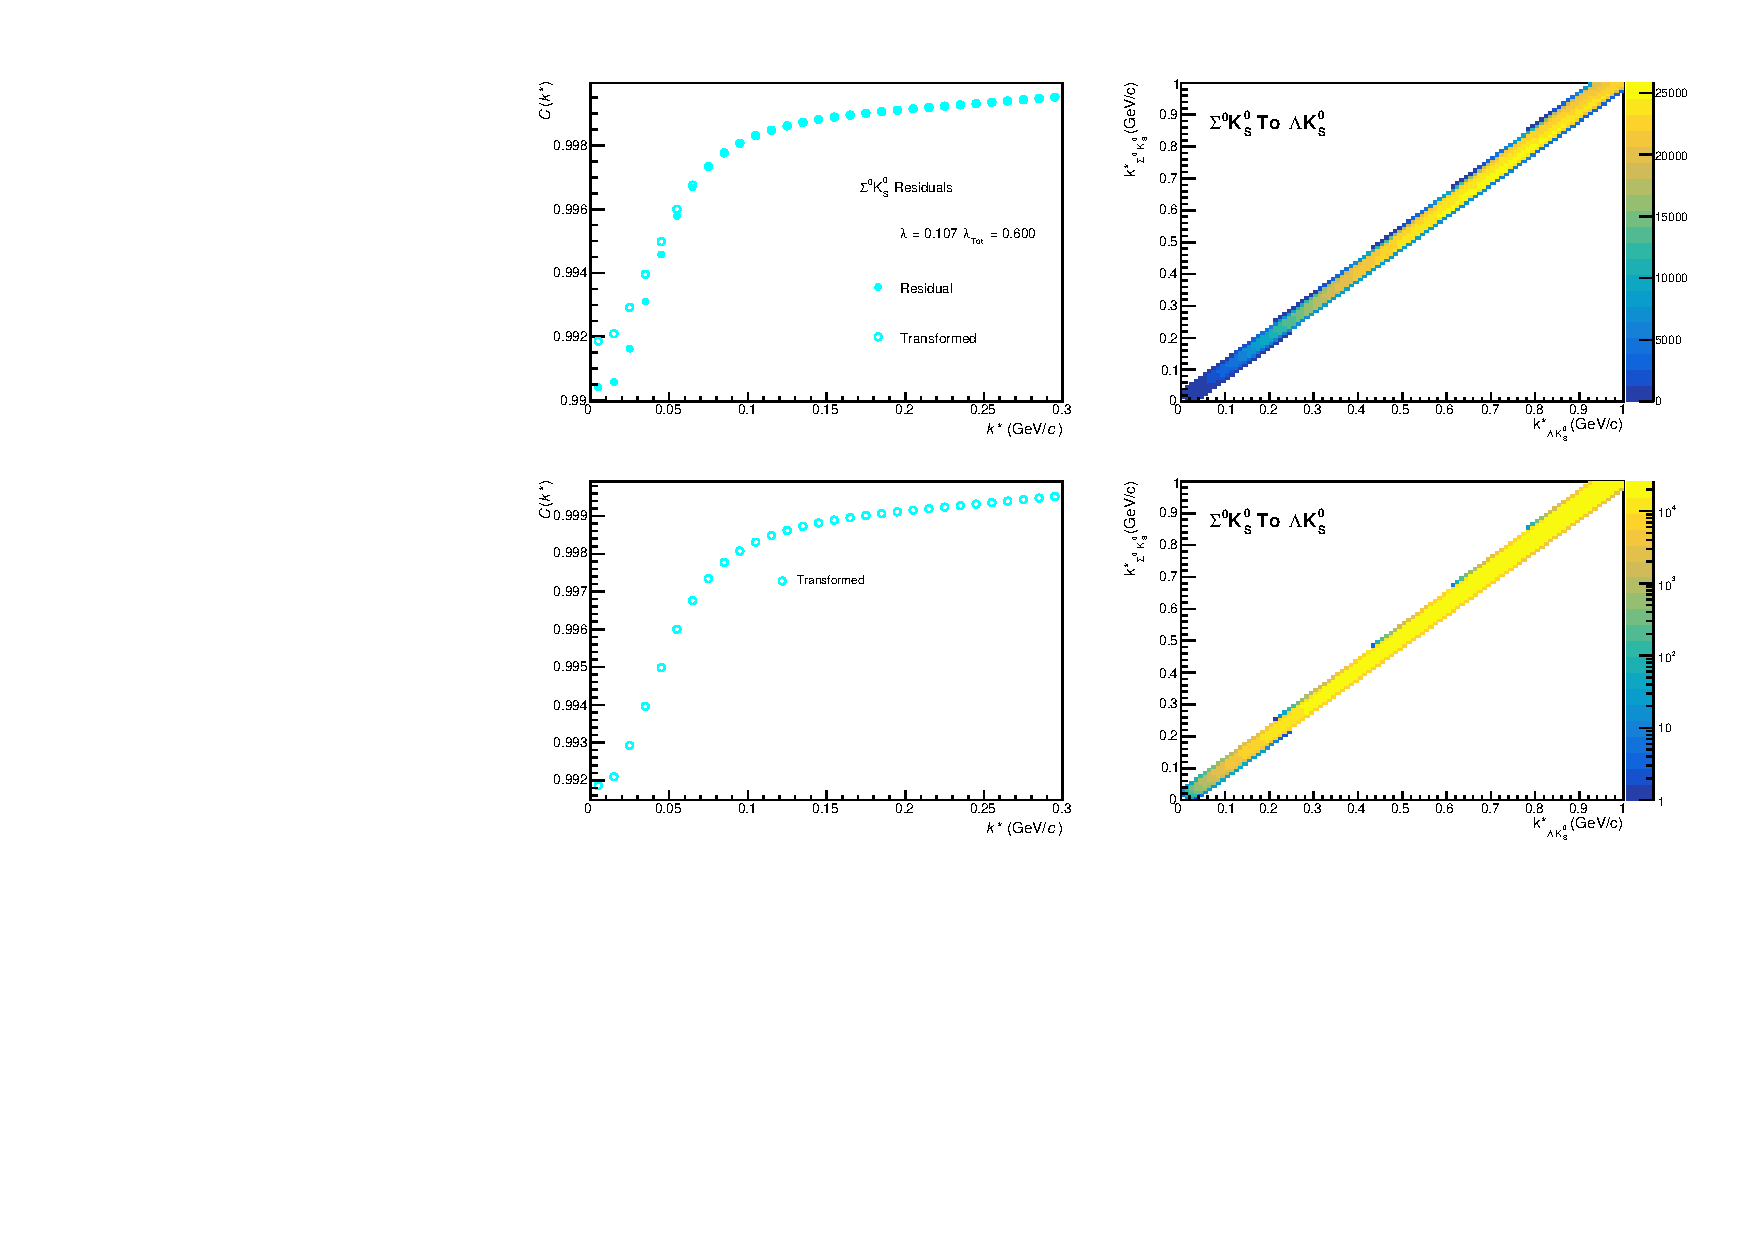
\includegraphics[width=\textwidth]{/home/jesse/Analysis/FemtoAnalysis/AnalysisNotes/Appendices/Appendix_AdditionalFigures/Figures/Residuals/LamK0/Residuals_LamK0_0010_Sig0K0_MomResCrctn_NonFlatBgdCrctn_SingleLamParam_10Res_PrimMaxDecay4fm_UsingXiDataAndCoulombOnly.pdf}
  \caption[Residuals: $\Sigma^{0}$K$^{0}_{S}$ to $\Lambda$K$^{0}_{S}$ (0-10\% Centrality)]{Residuals: $\Sigma^{0}$K$^{0}_{S}$ to $\Lambda$K$^{0}_{S}$ (0-10\% Centrality)}
  \label{fig:Res_LamK0_0010_Sig0K0}
\end{figure}


\begin{figure}[h]
  \centering
  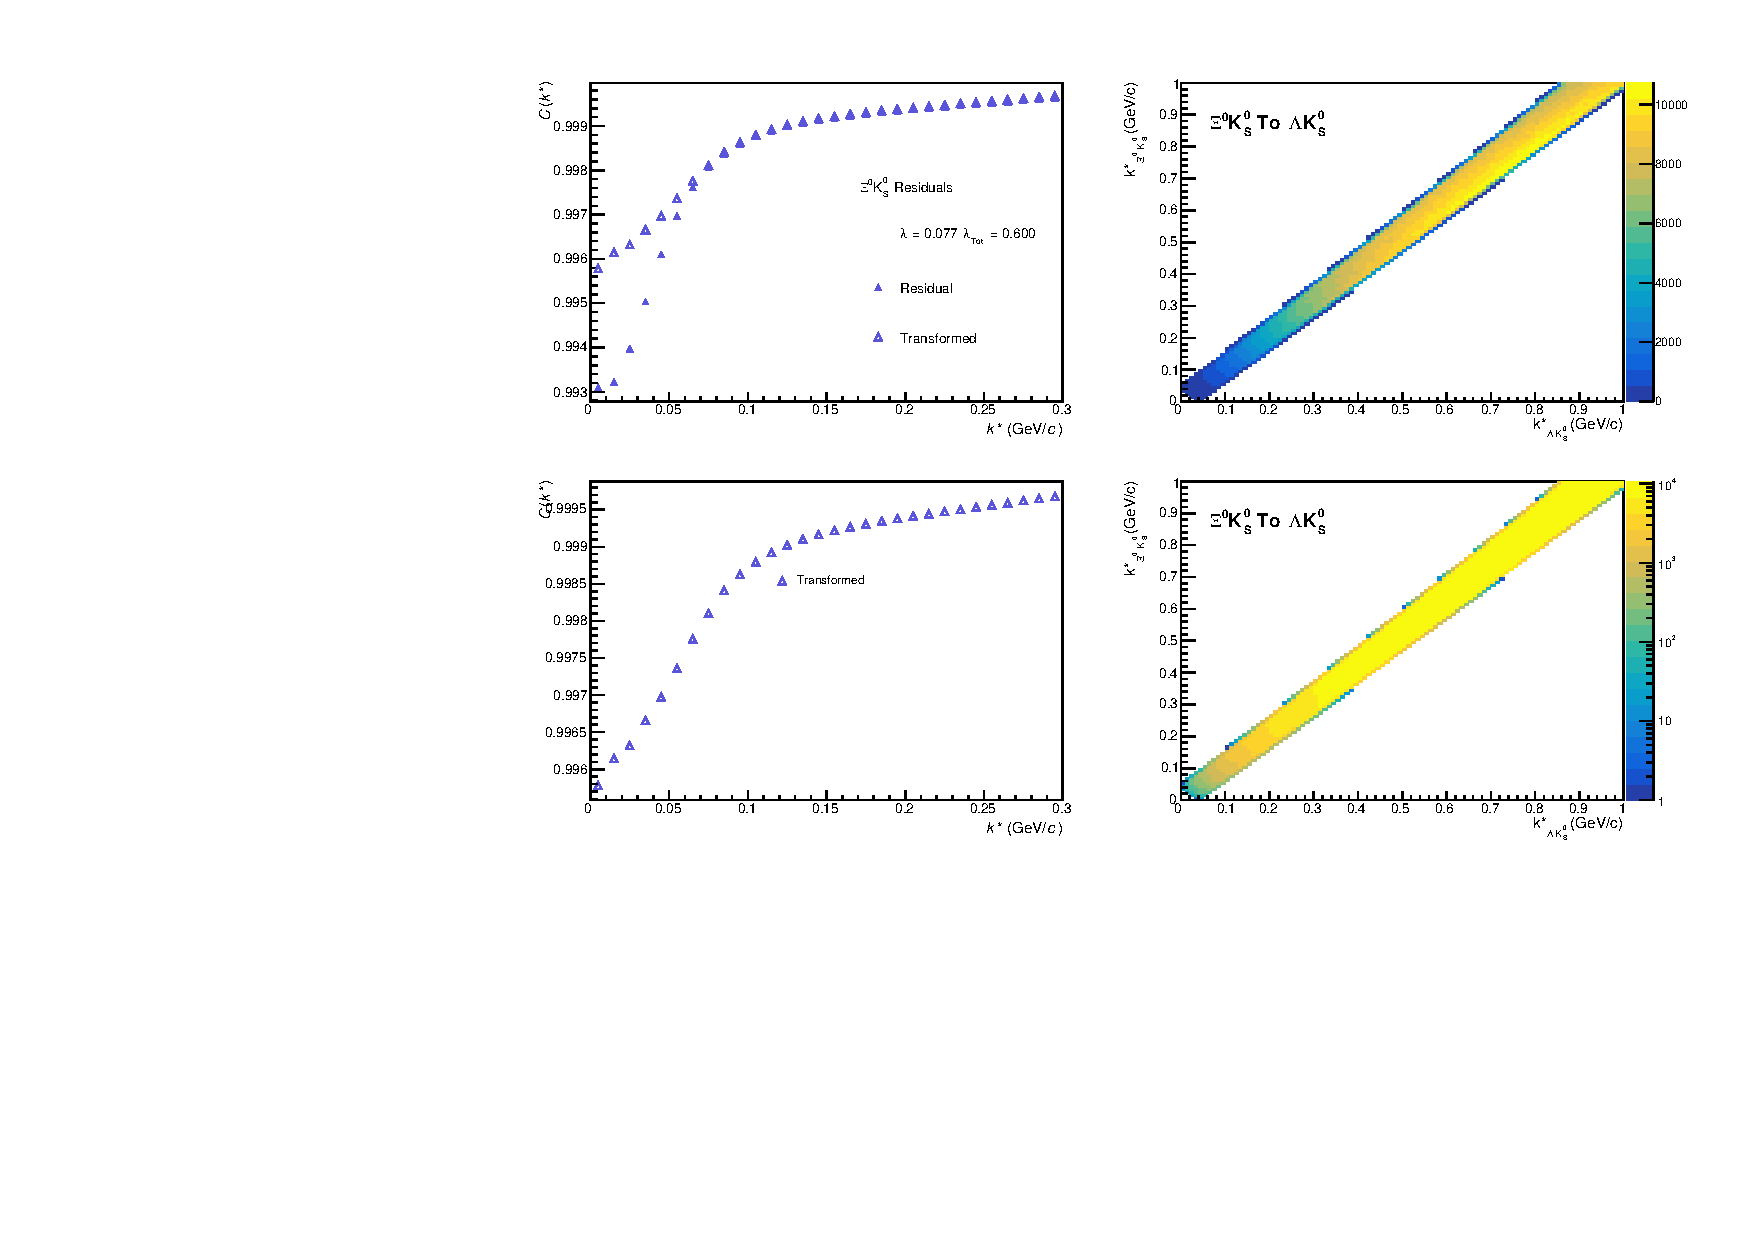
\includegraphics[width=\textwidth]{/home/jesse/Analysis/FemtoAnalysis/AnalysisNotes/Appendices/Appendix_AdditionalFigures/Figures/Residuals/LamK0/Residuals_LamK0_0010_Xi0K0_MomResCrctn_NonFlatBgdCrctn_SingleLamParam_10Res_PrimMaxDecay4fm_UsingXiDataAndCoulombOnly.pdf}
  \caption[Residuals: $\Xi^{0}$K$^{0}_{S}$ to $\Lambda$K$^{0}_{S}$ (0-10\% Centrality)]{Residuals: $\Xi^{0}$K$^{0}_{S}$ to $\Lambda$K$^{0}_{S}$ (0-10\% Centrality)}
  \label{fig:Res_LamK0_0010_Xi0K0}
\end{figure}


\begin{figure}[h]
  \centering
  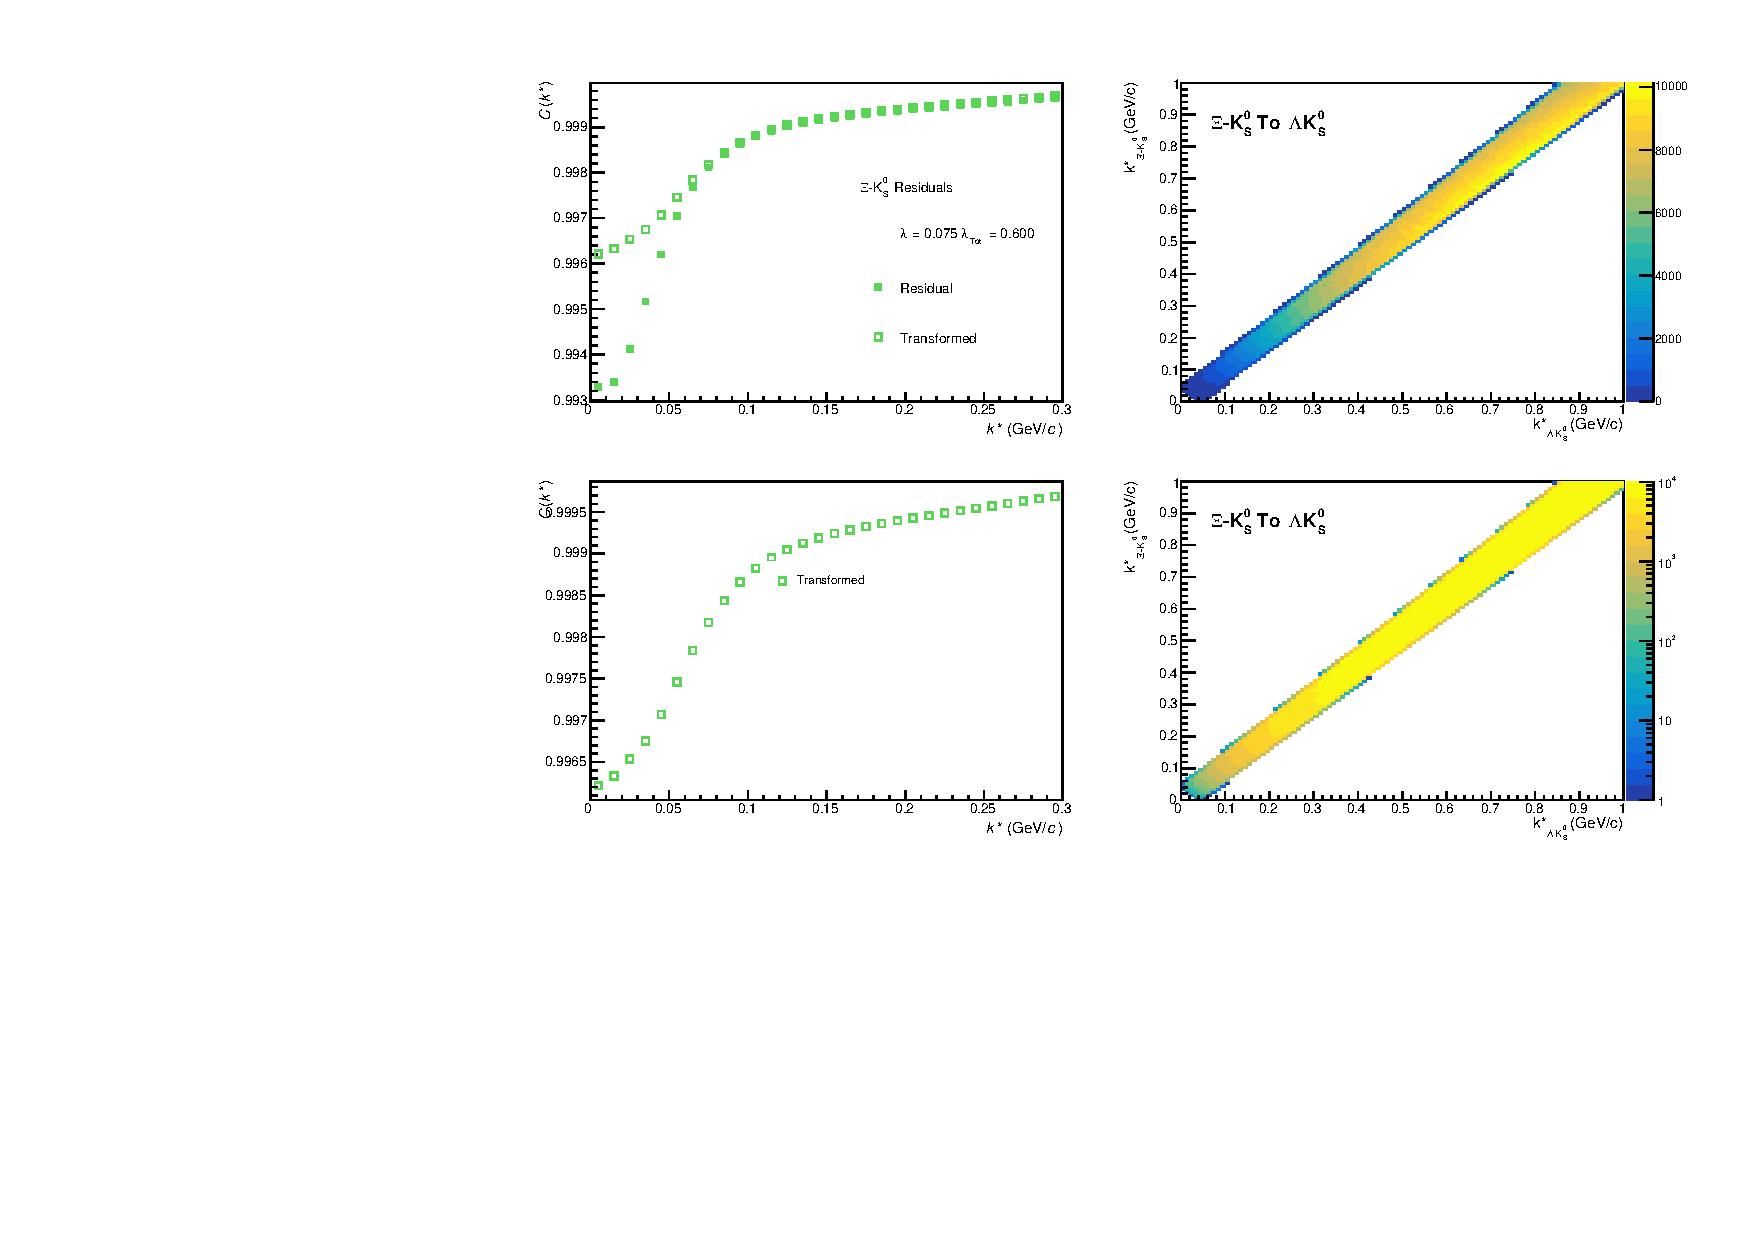
\includegraphics[width=\textwidth]{/home/jesse/Analysis/FemtoAnalysis/AnalysisNotes/Appendices/Appendix_AdditionalFigures/Figures/Residuals/LamK0/Residuals_LamK0_0010_XiK0_MomResCrctn_NonFlatBgdCrctn_SingleLamParam_10Res_PrimMaxDecay4fm_UsingXiDataAndCoulombOnly.pdf}
  \caption[Residuals: $\Xi^{-}$K$^{0}_{S}$ to $\Lambda$K$^{0}_{S}$ (0-10\% Centrality)]{Residuals: $\Xi^{-}$K$^{0}_{S}$ to $\Lambda$K$^{0}_{S}$ (0-10\% Centrality)}
  \label{fig:Res_LamK0_0010_XiCK0}
\end{figure}


\begin{figure}[h]
  \centering
  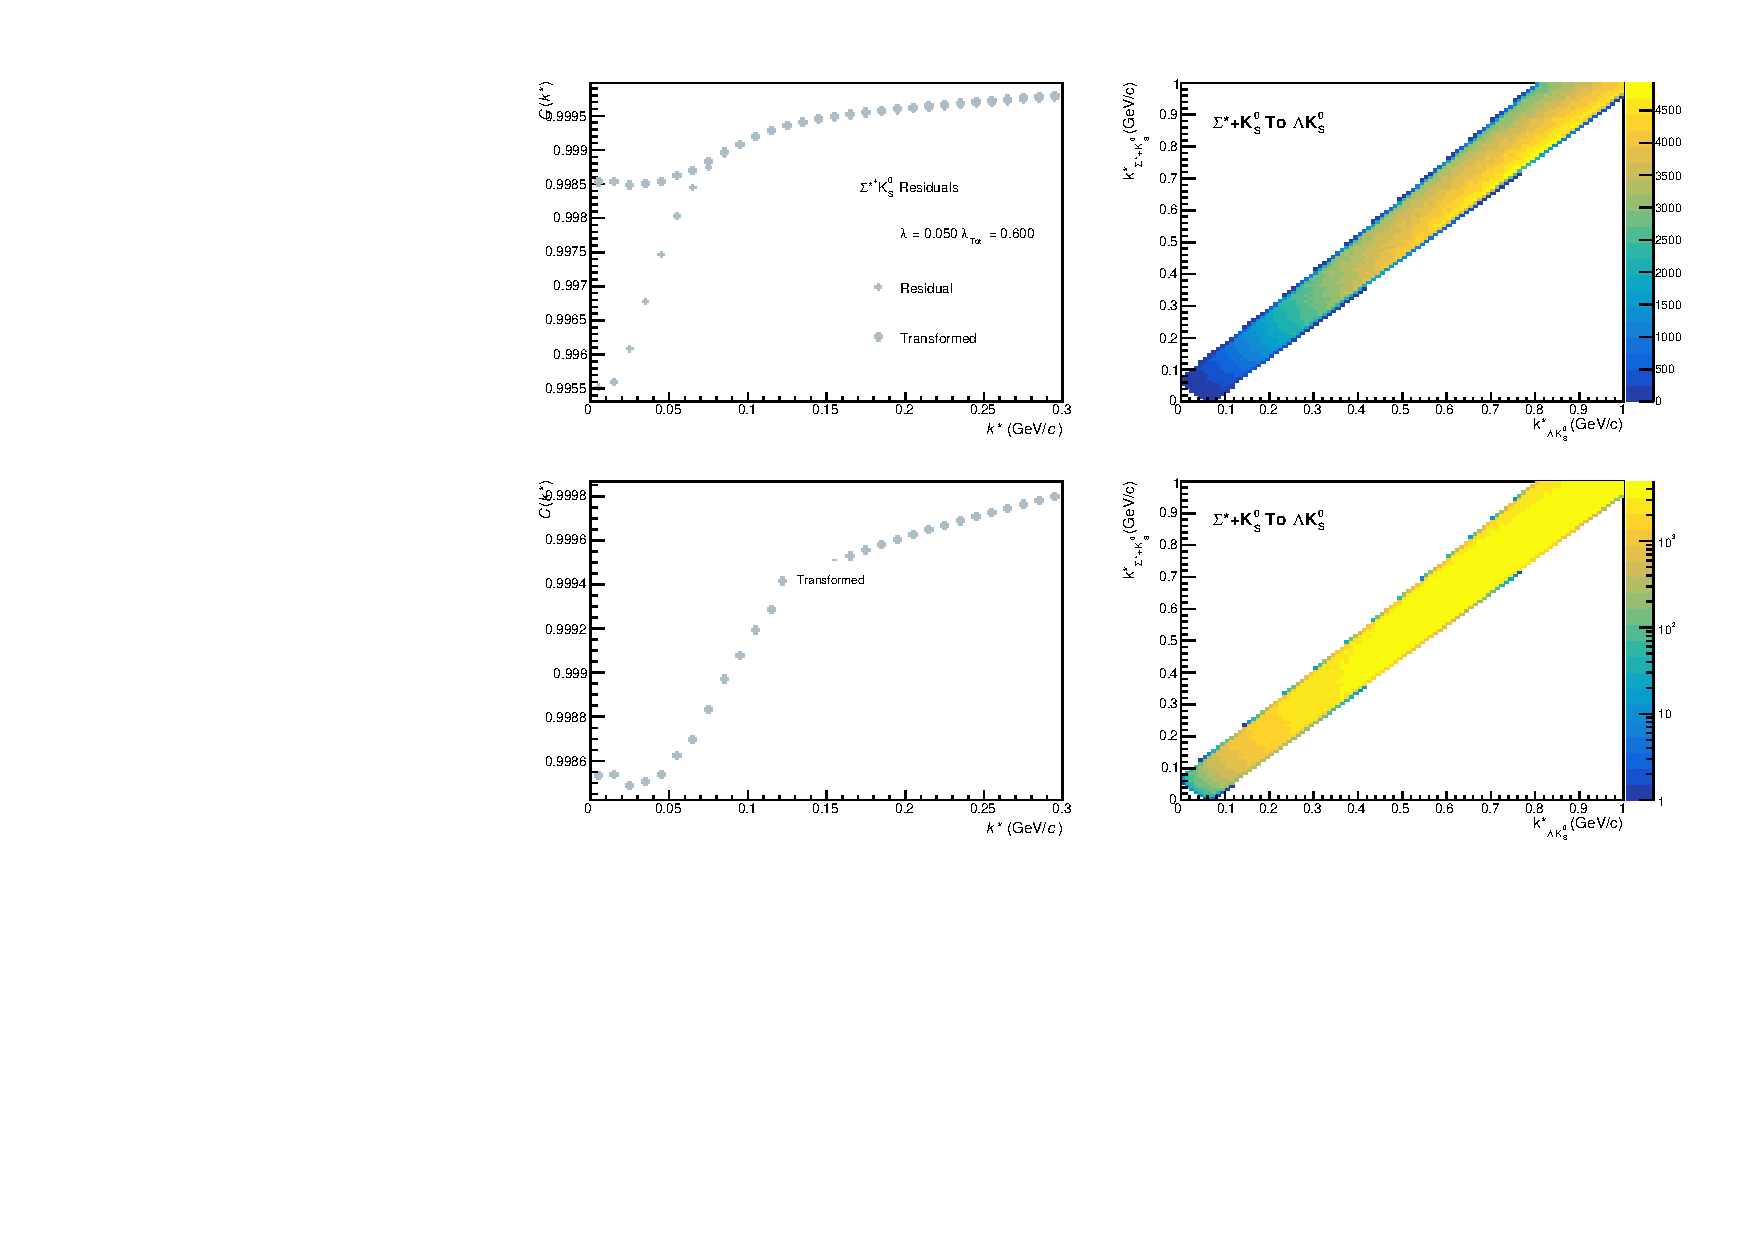
\includegraphics[width=\textwidth]{/home/jesse/Analysis/FemtoAnalysis/AnalysisNotes/Appendices/Appendix_AdditionalFigures/Figures/Residuals/LamK0/Residuals_LamK0_0010_SigStPK0_MomResCrctn_NonFlatBgdCrctn_SingleLamParam_10Res_PrimMaxDecay4fm_UsingXiDataAndCoulombOnly.pdf}
  \caption[Residuals: $\Sigma^{*+}$K$^{0}_{S}$ to $\Lambda$K$^{0}_{S}$ (0-10\% Centrality)]{Residuals: $\Sigma^{*+}$K$^{0}_{S}$ to $\Lambda$K$^{0}_{S}$ (0-10\% Centrality)}
  \label{fig:Res_LamK0_0010_SigStPK0}
\end{figure}

\begin{figure}[h]
  \centering
  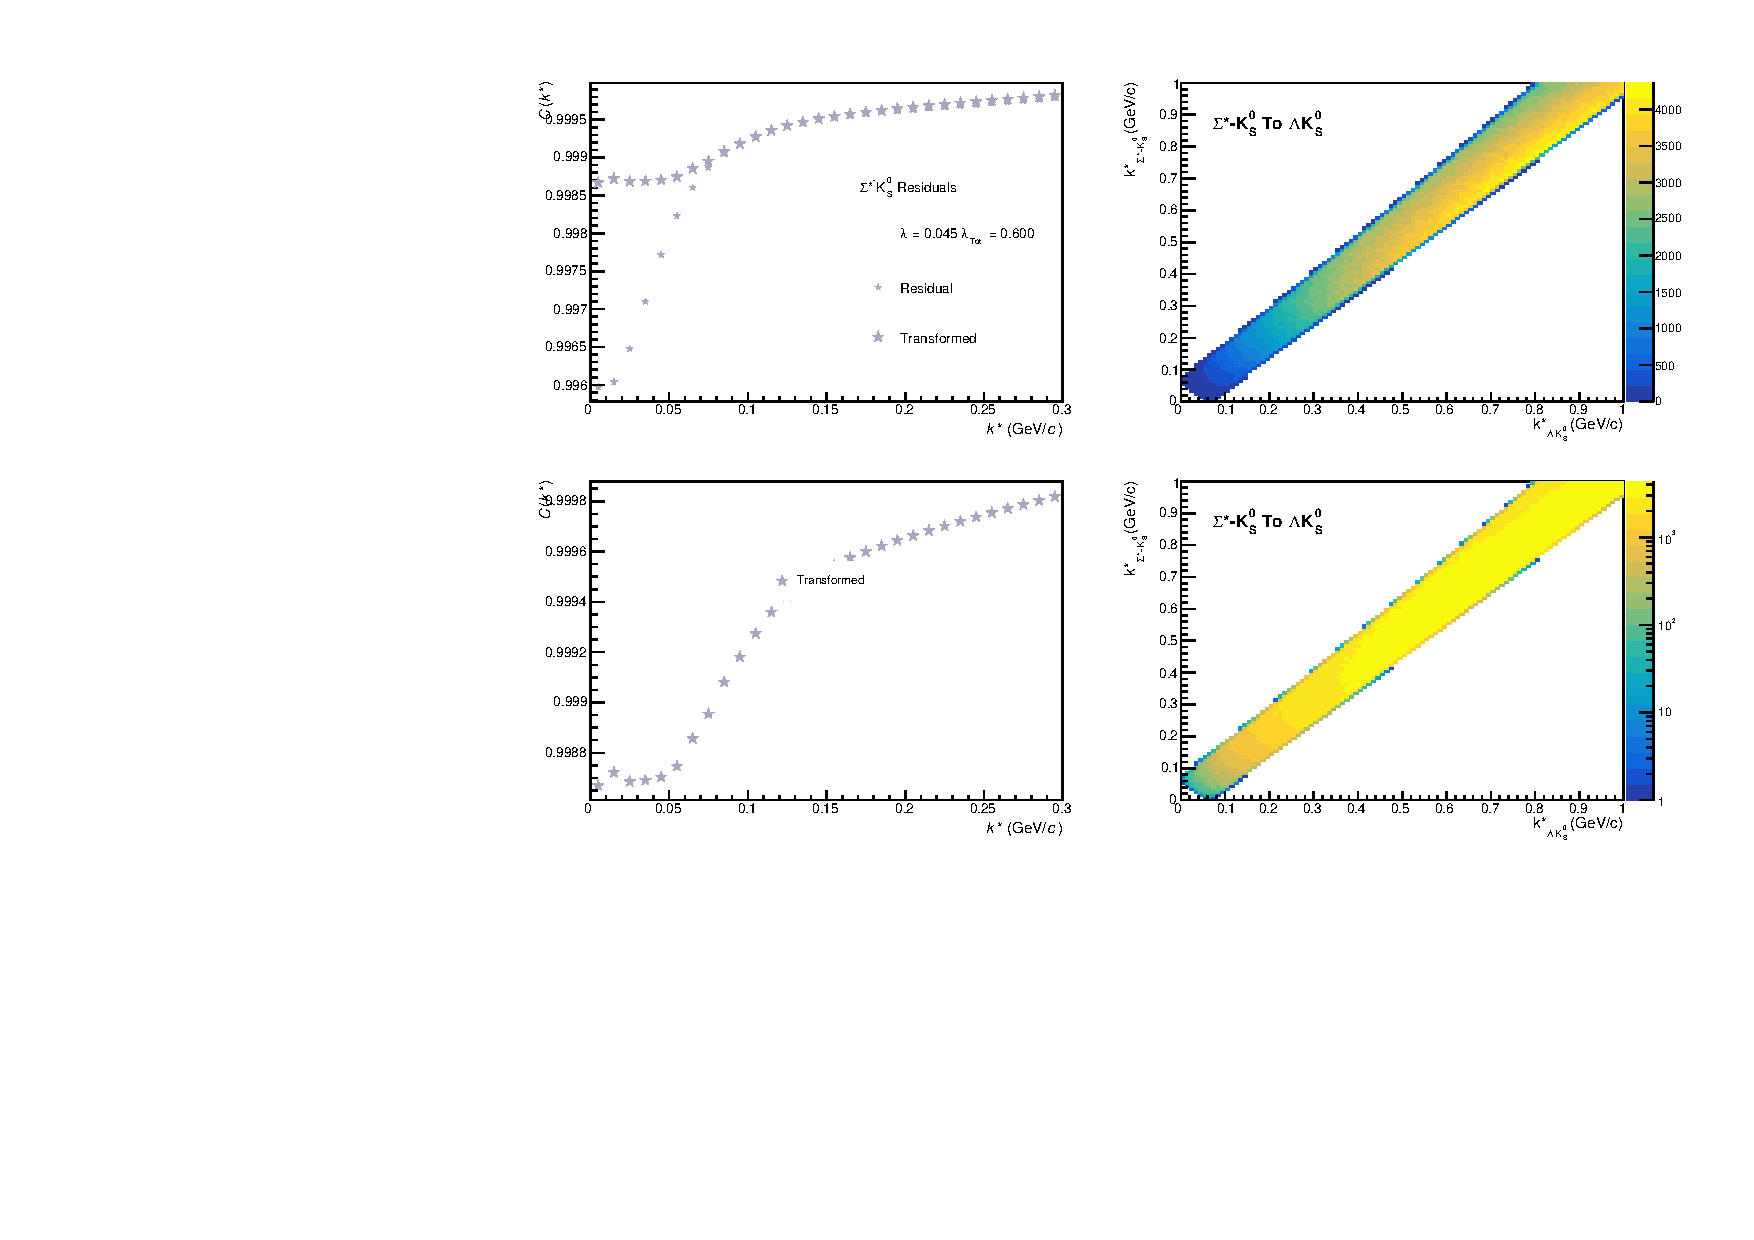
\includegraphics[width=\textwidth]{/home/jesse/Analysis/FemtoAnalysis/AnalysisNotes/Appendices/Appendix_AdditionalFigures/Figures/Residuals/LamK0/Residuals_LamK0_0010_SigStMK0_MomResCrctn_NonFlatBgdCrctn_SingleLamParam_10Res_PrimMaxDecay4fm_UsingXiDataAndCoulombOnly.pdf}
  \caption[Residuals: $\Sigma^{*-}$K$^{0}_{S}$ to $\Lambda$K$^{0}_{S}$ (0-10\% Centrality)]{Residuals: $\Sigma^{*-}$K$^{0}_{S}$ to $\Lambda$K$^{0}_{S}$ (0-10\% Centrality)}
  \label{fig:Res_LamK0_0010_SigStMK0}
\end{figure}

\begin{figure}[h]
  \centering
  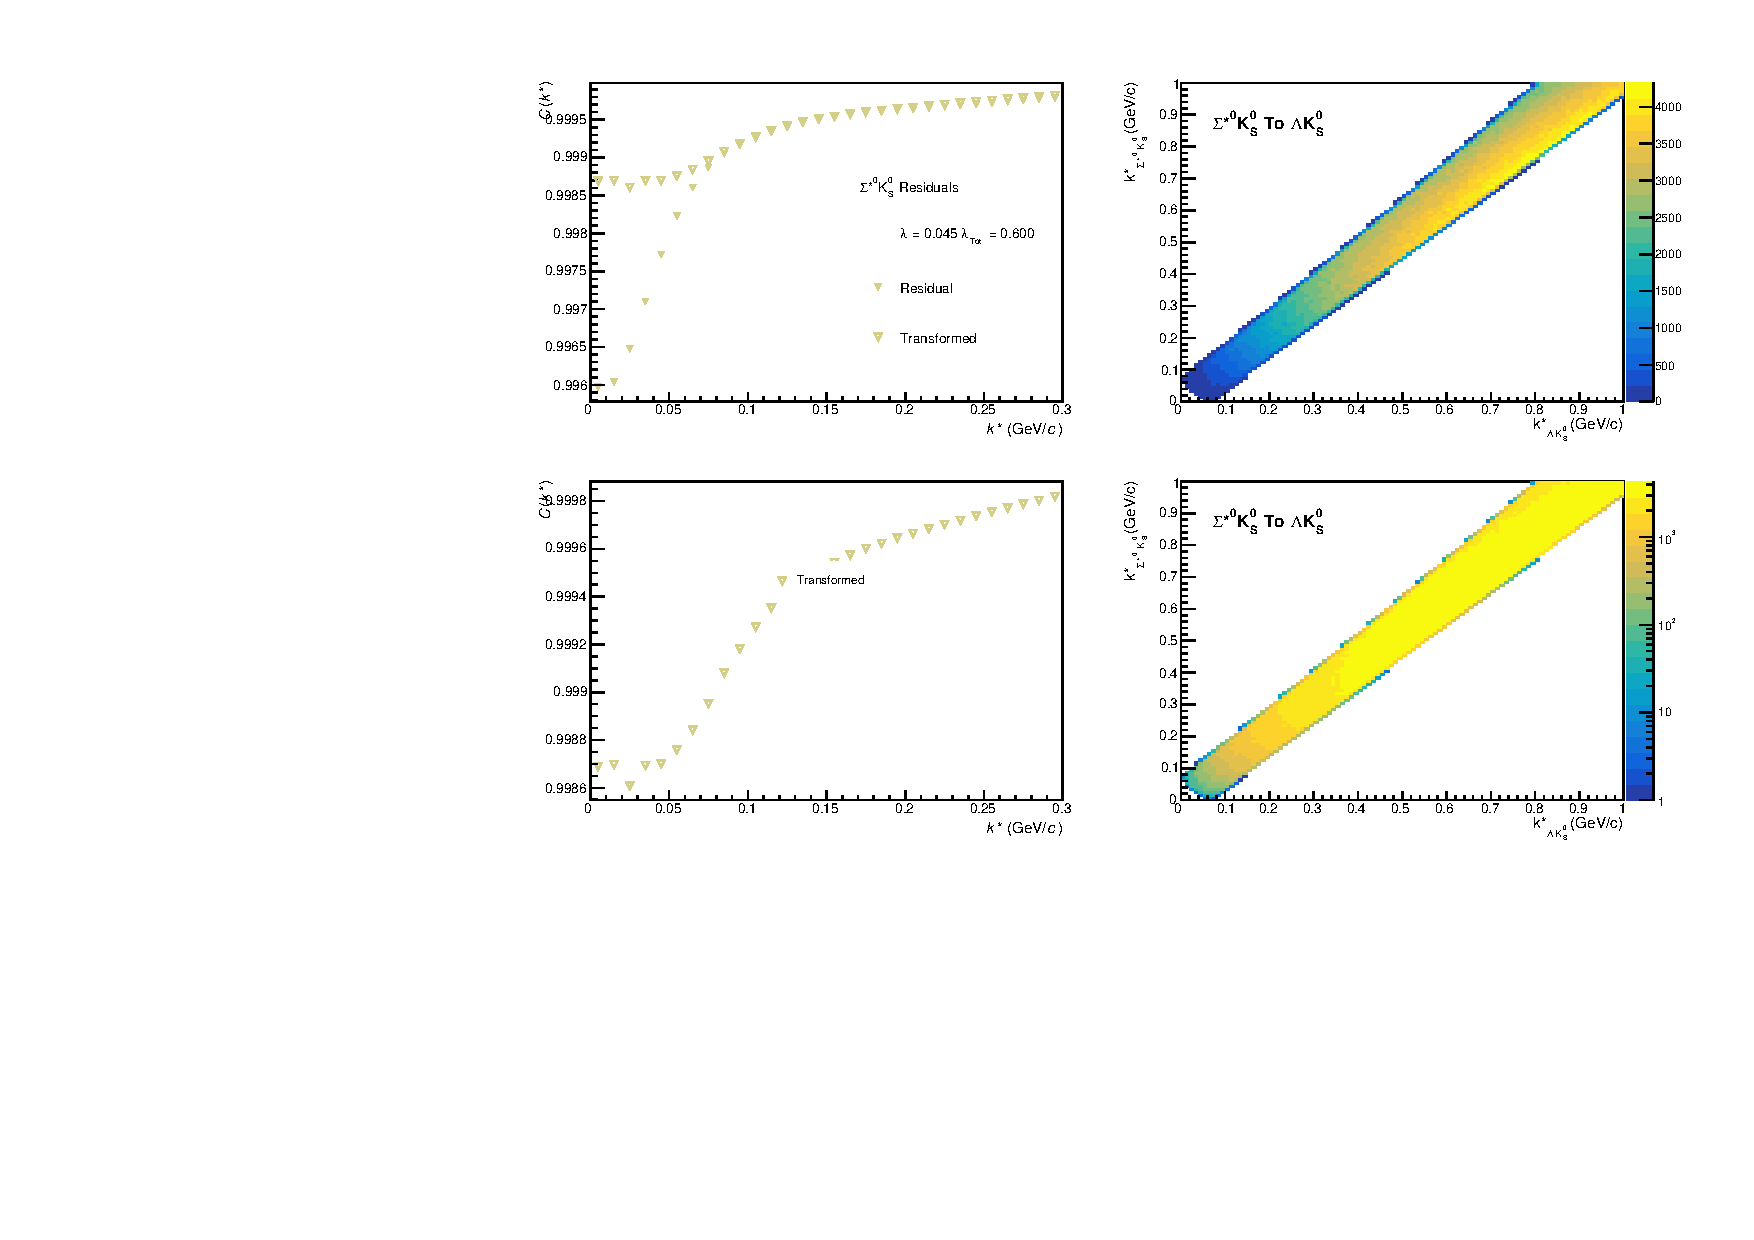
\includegraphics[width=\textwidth]{/home/jesse/Analysis/FemtoAnalysis/AnalysisNotes/Appendices/Appendix_AdditionalFigures/Figures/Residuals/LamK0/Residuals_LamK0_0010_SigSt0K0_MomResCrctn_NonFlatBgdCrctn_SingleLamParam_10Res_PrimMaxDecay4fm_UsingXiDataAndCoulombOnly.pdf}
  \caption[Residuals: $\Sigma^{*0}$K$^{0}_{S}$ to $\Lambda$K$^{0}_{S}$ (0-10\% Centrality)]{Residuals: $\Sigma^{*0}$K$^{0}_{S}$ to $\Lambda$K$^{0}_{S}$ (0-10\% Centrality)}
  \label{fig:Res_LamK0_0010_SigSt0K0}
\end{figure}


\begin{figure}[h]
  \centering
  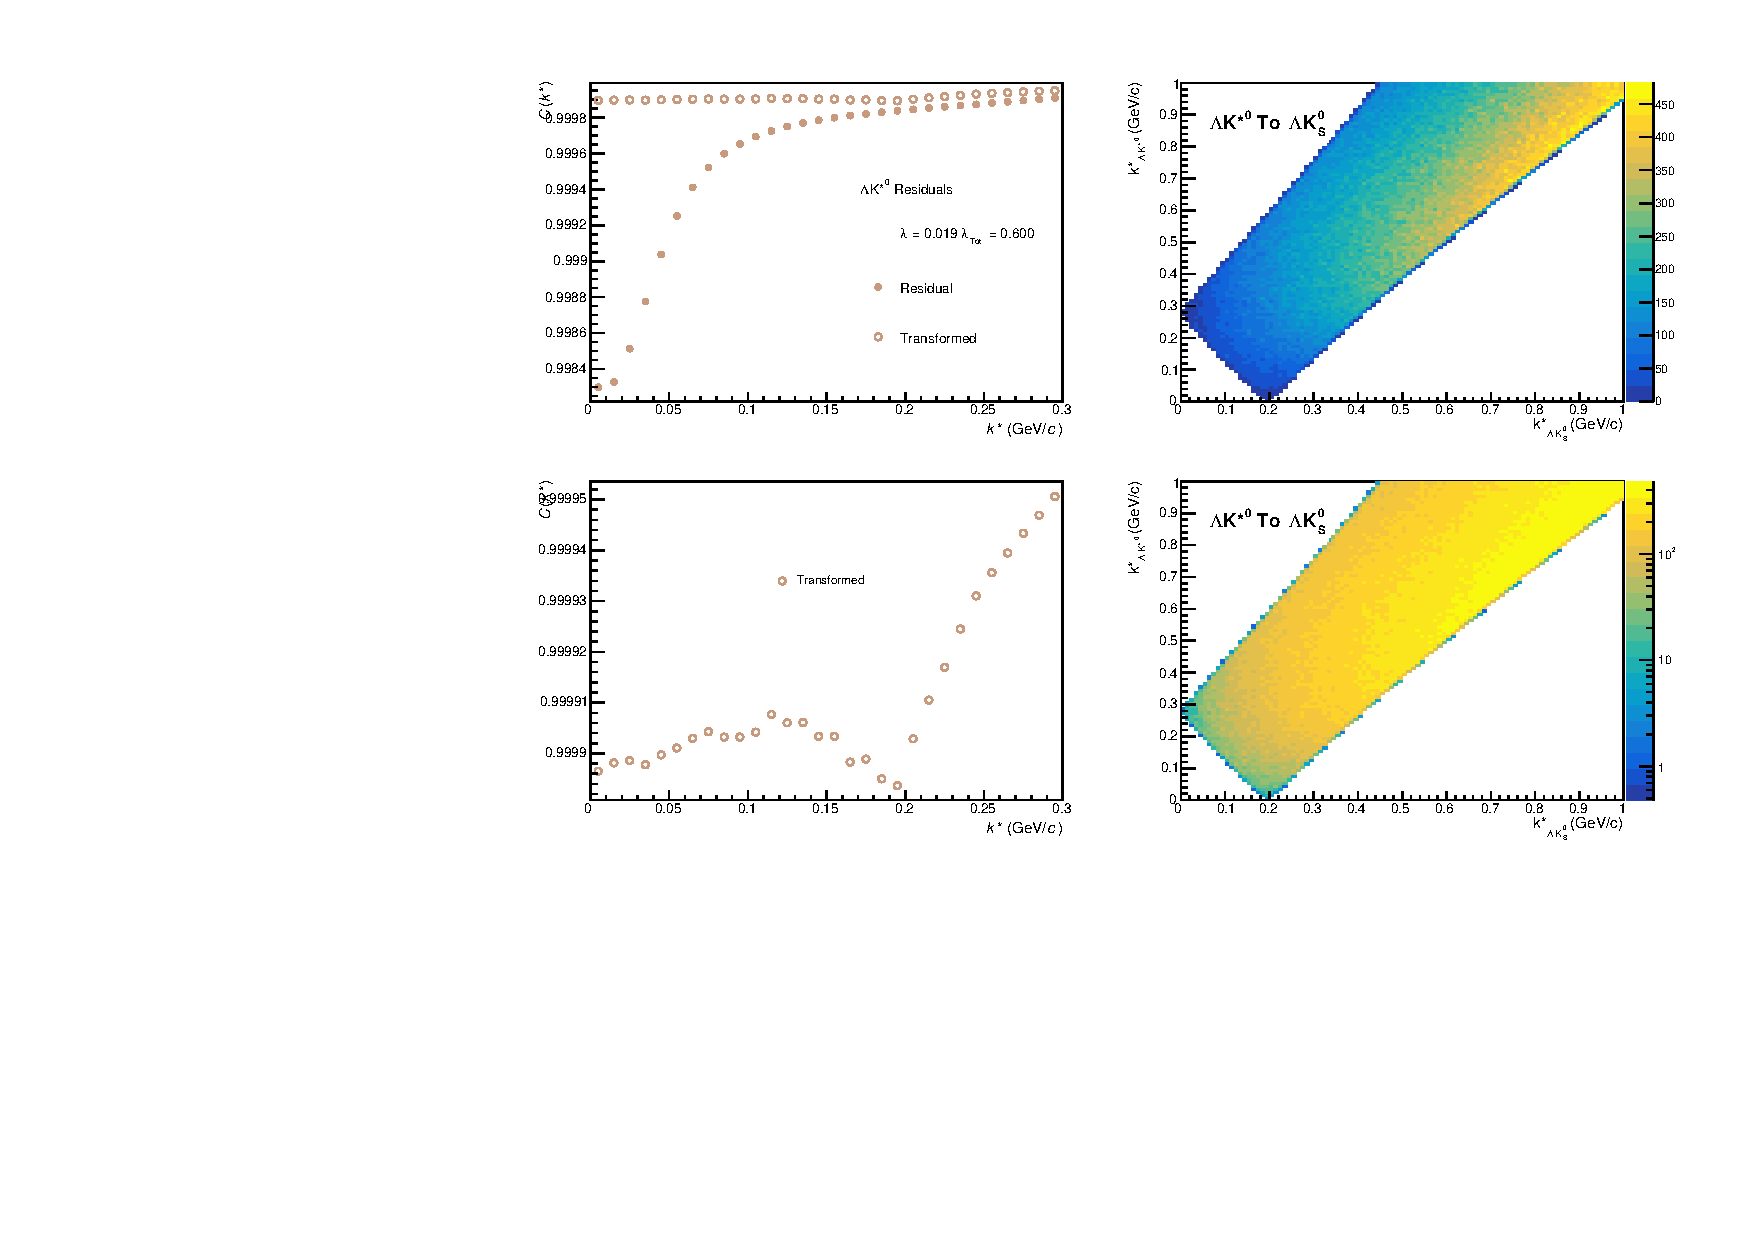
\includegraphics[width=\textwidth]{/home/jesse/Analysis/FemtoAnalysis/AnalysisNotes/Appendices/Appendix_AdditionalFigures/Figures/Residuals/LamK0/Residuals_LamK0_0010_LamKSt0ToLamK0_MomResCrctn_NonFlatBgdCrctn_SingleLamParam_10Res_PrimMaxDecay4fm_UsingXiDataAndCoulombOnly.pdf}
  \caption[Residuals: $\Lambda$K$^{*0}$ to $\Lambda$K$^{0}_{S}$ (0-10\% Centrality)]{Residuals: $\Lambda$K$^{*0}$ to $\Lambda$K$^{0}_{S}$ (0-10\% Centrality)}
  \label{fig:Res_LamK0_0010_LamKSt0}
\end{figure}


\begin{figure}[h]
  \centering
  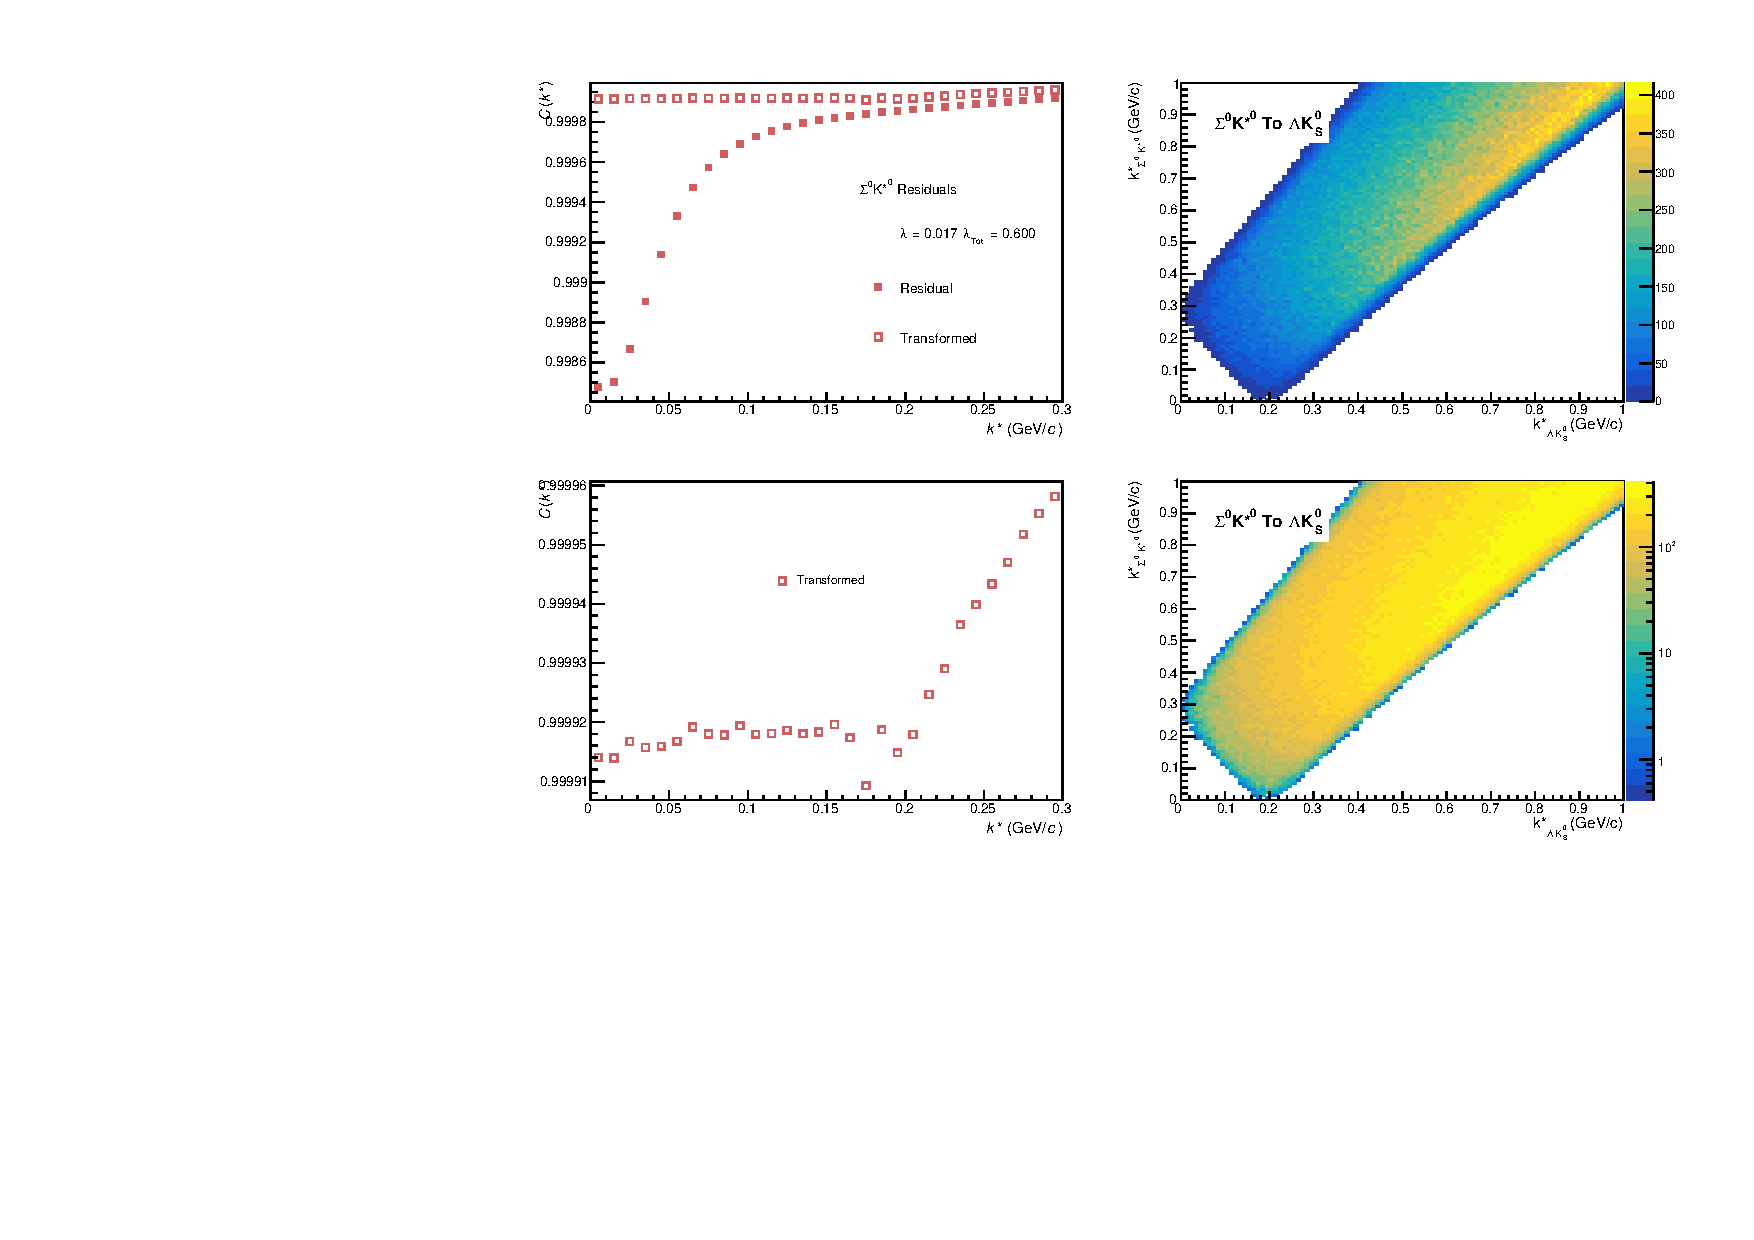
\includegraphics[width=\textwidth]{/home/jesse/Analysis/FemtoAnalysis/AnalysisNotes/Appendices/Appendix_AdditionalFigures/Figures/Residuals/LamK0/Residuals_LamK0_0010_Sig0KSt0ToLamK0_MomResCrctn_NonFlatBgdCrctn_SingleLamParam_10Res_PrimMaxDecay4fm_UsingXiDataAndCoulombOnly.pdf}
  \caption[Residuals: $\Sigma^{0}$K$^{*0}$ to $\Lambda$K$^{0}_{S}$ (0-10\% Centrality)]{Residuals: $\Sigma^{0}$K$^{*0}$ to $\Lambda$K$^{0}_{S}$ (0-10\% Centrality)}
  \label{fig:Res_LamK0_0010_Sig0KSt0}
\end{figure}


\begin{figure}[h]
  \centering
  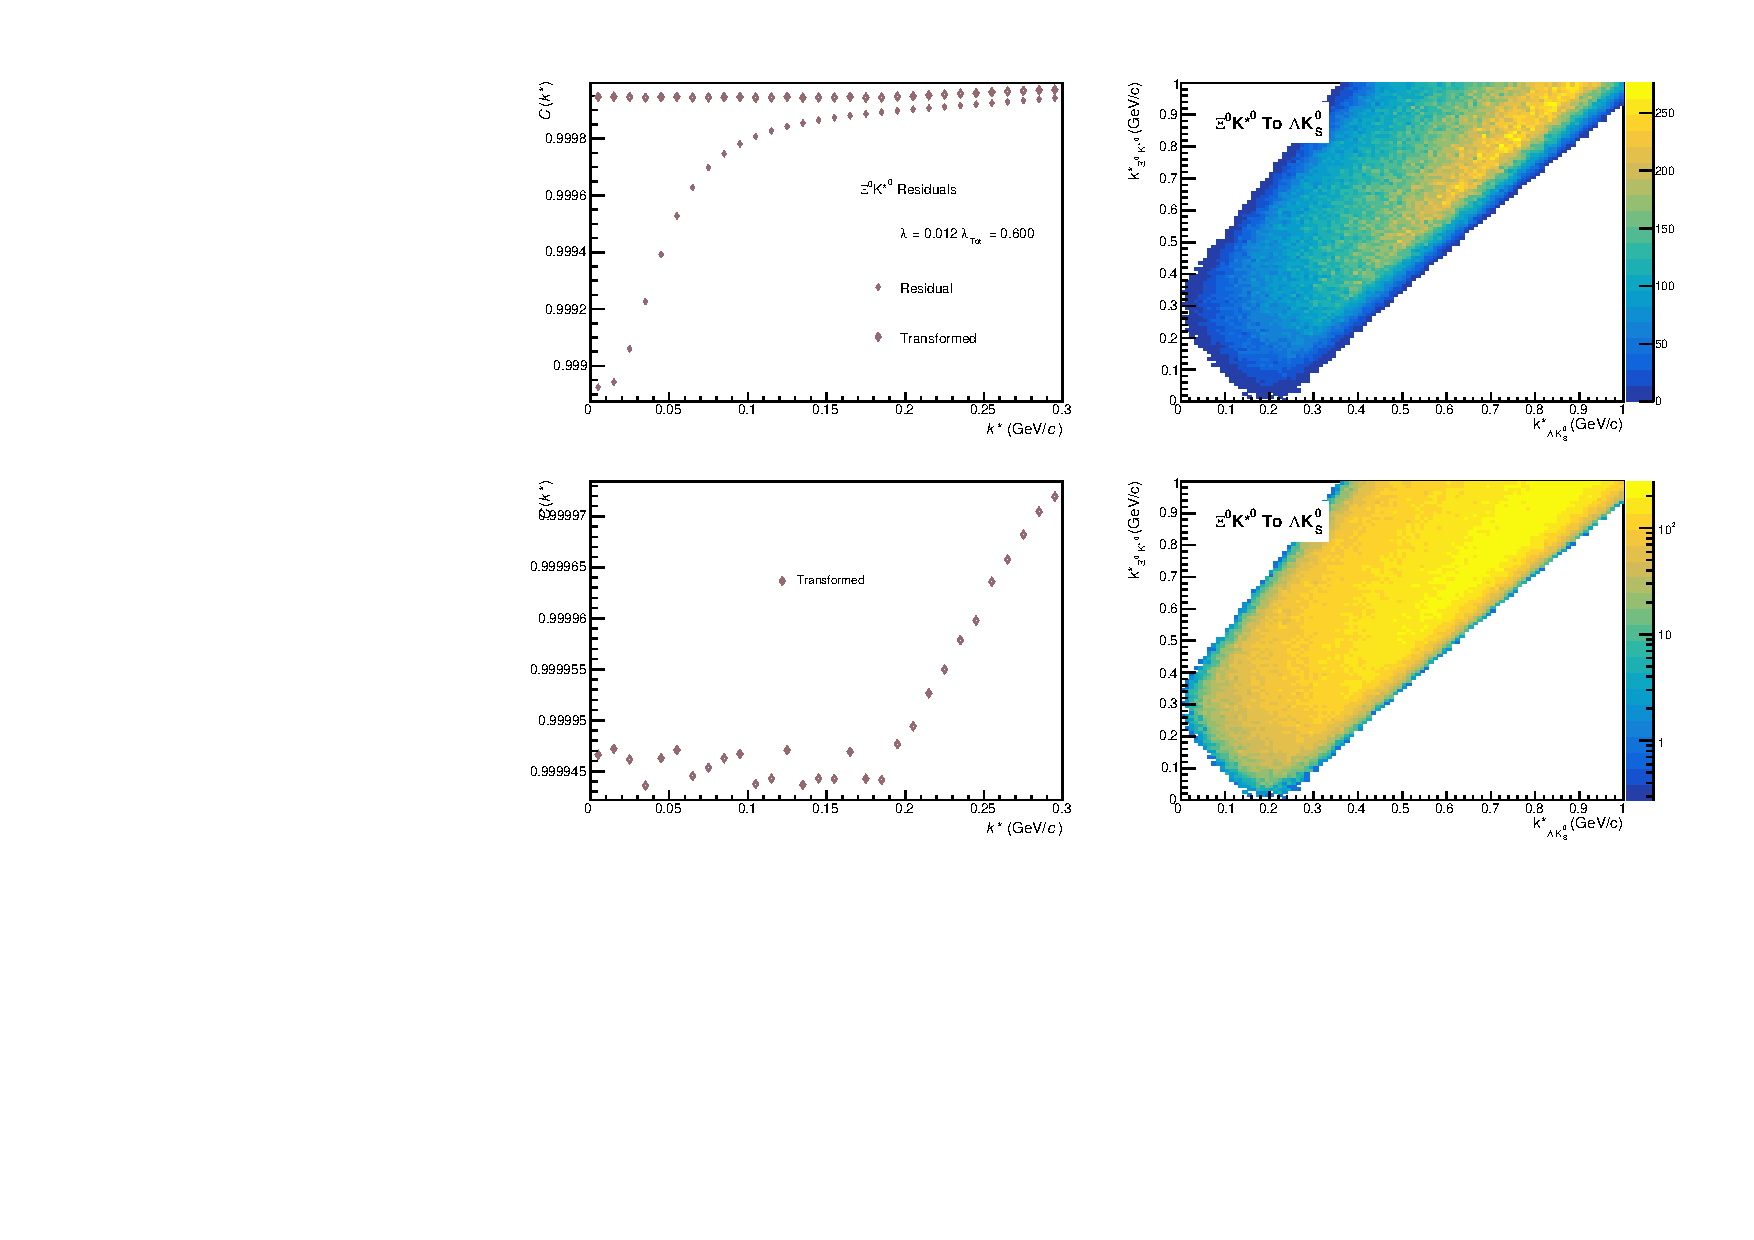
\includegraphics[width=\textwidth]{/home/jesse/Analysis/FemtoAnalysis/AnalysisNotes/Appendices/Appendix_AdditionalFigures/Figures/Residuals/LamK0/Residuals_LamK0_0010_Xi0KSt0ToLamK0_MomResCrctn_NonFlatBgdCrctn_SingleLamParam_10Res_PrimMaxDecay4fm_UsingXiDataAndCoulombOnly.pdf}
  \caption[Residuals: $\Xi^{0}$K$^{*0}$ to $\Lambda$K$^{0}_{S}$ (0-10\% Centrality)]{Residuals: $\Xi^{0}$K$^{*0}$ to $\Lambda$K$^{0}_{S}$ (0-10\% Centrality)}
  \label{fig:Res_LamK0_0010_Xi0KSt0}
\end{figure}

\begin{figure}[h]
  \centering
  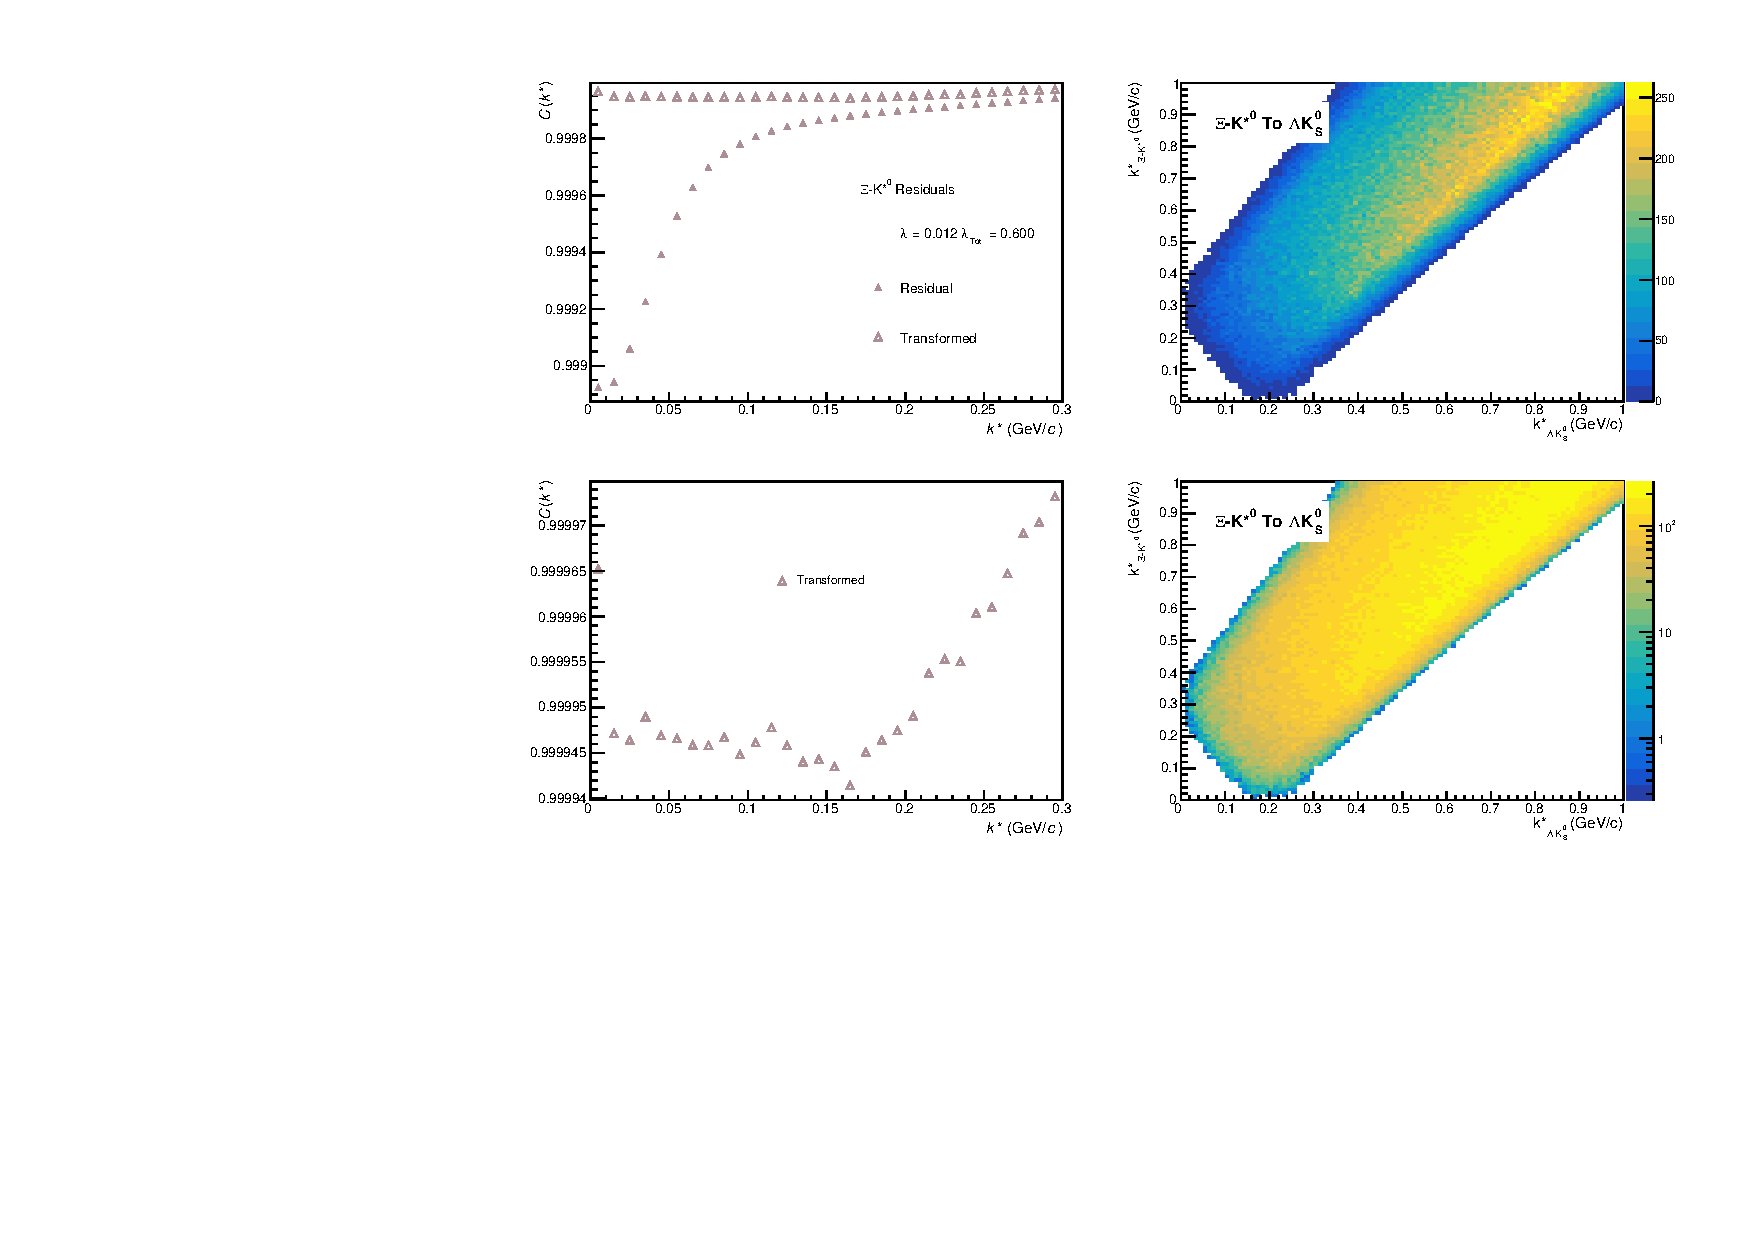
\includegraphics[width=\textwidth]{/home/jesse/Analysis/FemtoAnalysis/AnalysisNotes/Appendices/Appendix_AdditionalFigures/Figures/Residuals/LamK0/Residuals_LamK0_0010_XiKSt0ToLamK0_MomResCrctn_NonFlatBgdCrctn_SingleLamParam_10Res_PrimMaxDecay4fm_UsingXiDataAndCoulombOnly.pdf}
  \caption[Residuals: $\Xi^{-}$K$^{*0}$ to $\Lambda$K$^{0}_{S}$ (0-10\% Centrality)]{Residuals: $\Xi^{-}$K$^{*0}$ to $\Lambda$K$^{0}_{S}$ (0-10\% Centrality)}
  \label{fig:Res_LamK0_0010_XiCKSt0}
\end{figure}

\end{document}